% \documentclass[twoside, a4paper, draft]{article}
 \documentclass[twoside, a4paper]{article}

%	A header file that makes it easy to produce common mathematical operations,
%	such as the partial derivatives, curl, div etc...

\newcommand{\gv}[1]{\ensuremath{\mbox{\boldmath$ #1 $}}} 			% for vectors of Greek letters
\newcommand{\uv}[1]{\ensuremath{\mathbf{\hat{#1}}}} 				% for unit vector
\newcommand{\abs}[1]{\left| #1 \right|} 							% for absolute value
\newcommand{\avg}[1]{\left< #1 \right>} 							% for average

\let\underdot=\d 													% rename builtin command \d{} to \underdot{}
\renewcommand{\d}[2]{\frac{d #1}{d #2}} 							% for derivatives
\newcommand{\dd}[2]{\frac{d^2 #1}{d #2^2}}							% for double derivatives
\newcommand{\pd}[2]{\frac{\partial #1}{\partial #2}} 				% for partial derivatives
\newcommand{\pdd}[2]{\frac{\partial^2 #1}{\partial #2^2}} 			% for double partial derivatives
\newcommand{\pDD}[3]{\frac{\partial^2 #1}{\partial #2 \partial #3}}			% for double partial derivative w.r.t different variables
\newcommand{\pdc}[3]{\left( \frac{\partial #1}{\partial #2} \right)_{#3}} % for thermodynamic partial derivatives

\newcommand{\ket}[1]{\left| #1 \right>} 							% for Dirac bras
\newcommand{\bra}[1]{\left< #1 \right|} 							% for Dirac kets
\newcommand{\braket}[2]{\left< #1 \vphantom{#2} \right| \left. #2 \vphantom{#1} \right>} % for Dirac brackets
\newcommand{\matrixel}[3]{\left< #1 \vphantom{#2#3} \right| #2 \left| #3 \vphantom{#1#2} \right>} % for Dirac matrix elements

\newcommand{\grad}[1]{\nabla #1} 				% for gradient
\let\divsymb=\div 									% rename builtin command \div to \divsymb
\renewcommand{\div}[1]{\nabla \cdot \gv{#1}} 		% for divergence
\newcommand{\curl}[1]{\nabla \times \gv{#1}} 		% for curl
\let\baraccent=\= 									% rename builtin command \= to \baraccent
\renewcommand{\=}[1]{\stackrel{#1}{=}} 				% for putting numbers above =

\newcommand{\curlv}[1]{\curl{\vec{ #1 }}}			% curl with a vector symbol
\newcommand{\divv}[1]{\div{\vec{#1}}}				% div of a vector
\newcommand{\pdv}[2]{\pd{\gv{#1}}{#2}}				% partial derivative with a vector symbol
\newcommand{\pddv}[2]{\pdd{\gv{#1}}{#2}}			% 2nd partial derivative of a vector


% \usepackage{showlabels} % shows labels for figures
% \usepackage{showkeys}	% shows labels for equations

\usepackage{amsmath}
\usepackage{amssymb}
\usepackage{amsfonts}
\usepackage{verbatim}
\usepackage{cite}
\usepackage{setspace}
\usepackage{textcomp}
\usepackage{graphicx}
\usepackage{multirow}
%\usepackage[dvips]{graphicx}

\title{Coaxial Waveguide}
\author{Marko Milicevic}
\date{}	% Don't print the date
%\doublespacing
%\linespread{1.5}

\begin{document}
\maketitle
\pagenumbering{Roman}
\begin{abstract}
We find the expressions for the electric and magnetic fields, $\gv{E}$ and $\gv{H}$, inside a coaxial waveguide with perfectly conducting walls, using the results from ``Waveguide Equations''.
\end{abstract}

\tableofcontents
\newpage
\pagenumbering{arabic}
\section{Introduction}

We study the coaxial waveguide where the cross section is composed of two concentric circles with outer and inner radii $a$ and $b$ respectively. It is convenient to define the ratio $c = \frac{a}{b}$ for later equations. Positions within the cross section are described by the azimuthal angle $\phi$ and the distance from the centre $\rho$ (figure~\ref{fig:coaxial-waveguide}).

\begin{figure}[hbt]
	\centering
	\fbox{
	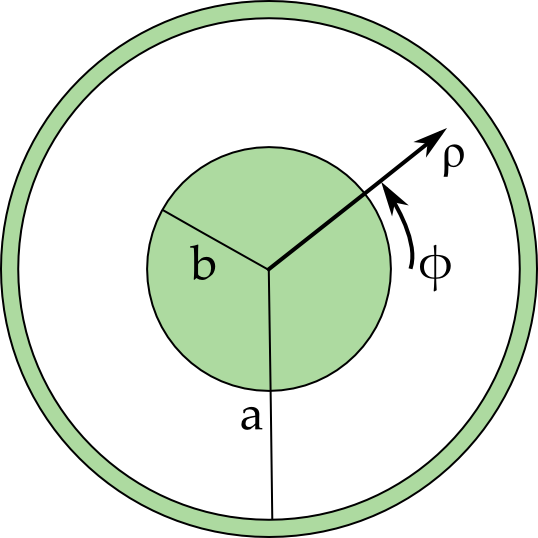
\includegraphics[width=75mm]{pic/coaxial_coordinates.png}
	}
	\caption{Coaxial waveguide cross section}
	\label{fig:coaxial-waveguide}
\end{figure} 

With this set of coordinates the displacement $d\gv{s}$ is given by
\begin{align*}
d\gv{s} = d\rho \, \hat{\rho} & + \rho \, d\phi \, \hat{\phi} + dz \, \hat{z}
\end{align*}
and we can use our results from ``Waveguide Equations'', with $h_1 = h_\rho = 1$, $h_2 = h_\phi = \rho$ and $h_3 = h_z = 1$.

\section{Scalar Field Equation}
\label{sec:phi}

The Electric and Magnetic fields are totally determined by the scalar field $\Phi$, which is found by solving the equation 
\begin{equation}
\label{eq:Phi}
\rho^2 \pdd{\Phi}{\rho} + \rho \pd{\Phi}{\rho} +
\rho^2 \pdd{\Phi}{z} + \epsilon \mu \omega^2 \rho^2 \Phi +
\pdd{\Phi}{\phi}
& = 0
\end{equation}
We assume that $\Phi$ can be written in the form
\begin{equation}
\label{eq:seperation-of-variables}
\Phi(\rho, \phi, z, t) = R(\rho) P(\phi) Z(z) \exp \left( i \omega t \right)
\end{equation}
Placing this in (\ref{eq:Phi}) gives
\begin{equation}
\label{eq:coaxial-function(rho,z)-equals-function(phi)}
\rho^2 \frac{R''}{R} + \rho \frac{R'}{R} + \rho^2 \frac{Z''}{Z} + 
\epsilon \mu \omega^2 \rho^2 
 = -\frac{P''}{P}
\end{equation}
where $R' = \d{R}{\rho}$, $Z' = \d{Z}{z}$ and $P' = \d{P}{\phi}$. \\
The left hand side of (\ref{eq:coaxial-function(rho,z)-equals-function(phi)}) is a function of $\rho$ and $z$, while the right hand side is a function of $\phi$. This can only be true if both sides are equal to a constant, which we'll label $m^2$. The right hand side of (\ref{eq:coaxial-function(rho,z)-equals-function(phi)}) becomes
\begin{align}
\label{eq:coaxial-P(phi)}
P''(\phi) & = -m^2 P(\phi) 
\nonumber \\
% % % % % % % % % % % %
P(\phi) & =\left\{
\begin{array}{l}
\cos( m \phi ) \\
\sin( m \phi )
\end{array}\right.
\quad m = 0, \, \pm 1, \, \pm 2, \, \pm 3 \, \ldots
\end{align}
where the values of $m$ are obtained  by noting that \mbox{$(\rho, \phi, z)$} and \mbox{$(\rho, \phi + 2 \pi, z)$} represent the same point in space \mbox{$\Rightarrow P(\phi) = P(\phi + 2 \pi)$}. \\
The left hand side of (\ref{eq:coaxial-function(rho,z)-equals-function(phi)}) is
\begin{align}
\label{eq:coaxial-function(rho)-equals-function(z)}
\rho^2 \frac{R''}{R} + \rho \frac{R'}{R} + \rho^2 \frac{Z''}{Z} + 
\epsilon \mu \omega^2 \rho^2 
& = m^2
\nonumber \\
\underbrace{
\frac{R''}{R} + \frac{1}{\rho} \frac{R'}{R} +
\epsilon \mu \omega^2 -\frac{m^2}{\rho^2} 
}_{\mbox{function of $\rho$}}
& = 
\underbrace{
-\frac{Z''}{Z}
}_{\mbox{function of $z$}}
\end{align}
which can only be true if both sides are equal to a constant, $k_z^2$. The right hand side of (\ref{eq:coaxial-function(rho)-equals-function(z)}) becomes
\begin{align}
\label{eq:coaxial-Z}
Z''(z) & = - k_z^2 Z(z)
\nonumber \\
Z(z) & = \exp( - i k_z z )
\end{align}
where we have chosen the solution for a wave travelling in the positive $z$ direction given an $\exp(i \omega t)$ time dependence. The left hand side of (\ref{eq:coaxial-function(rho)-equals-function(z)}) is
\begin{align}
\label{eq:R-ode}
\frac{R''}{R} + \frac{1}{\rho} \frac{R'}{R} +
\epsilon \mu \omega^2 -\frac{m^2}{\rho^2} 
& = k_z^2
\nonumber \\
\rho^2 R''( \rho ) + \rho R'( \rho ) + 
\left( 
\left( \frac{\chi}{b} \right) ^2 \rho^2 - m^2
\right)
R( \rho ) & = 0,
\quad \quad
\left( \frac{\chi}{b} \right)^2 = \epsilon \mu \omega^2 - k_z^2 
\end{align}
which is the form of Bessel's differential equation and has the solution
\begin{align}
\label{eq:coaxial-R}
R \left( \rho \right) & = A \, J_m \left( \frac{ \chi }{b}  \rho \right) + B \, Y_m \left( \frac{\chi}{b} \rho \right)
\end{align}
Where $A$ and $B$ are constants, $J_m$ and $Y_m$ are Bessel functions of the first and second kind of order $m$ and the factor $b$ has been placed in for convenience. In the case of a cylindrical cavity we discard $Y_m$ as a solution because $Y_m \rightarrow \infty \mbox{ as } \rho \rightarrow 0$, here we do not because our solution only spans \mbox{$b < \rho < a$}. Also this solution is only valid if $\chi \neq 0$, as (\ref{eq:R-ode}) is no longer in the form of Bessel's differential equation otherwise. In the case of $\chi = 0$ we get a special \textit{Transverse Electric Magnetic mode} (TEM) which will be discussed in section \ref{sec:TEM}.\\

Gathering (\ref{eq:coaxial-P(phi)}), (\ref{eq:coaxial-Z}) and (\ref{eq:coaxial-R}) into (\ref{eq:seperation-of-variables}), and setting $k^2 = \epsilon \mu \omega^2$, gives our solution for $\Phi$ as
\begin{align}
\label{eq:phi-solution}
\Phi & = 
\left[
A \, J_m \left( \frac{ \chi}{b} \rho \right) + B \, Y_m \left( \frac{ \chi }{b} \rho \right)
\right]
\left\{
\begin{array}{c}
\sin \left( m \phi \right) \\
\cos \left( m \phi \right)
\end{array}
\right\}
\exp i \left( \omega t -k_z z \right)\\
m & = 0, \, \pm 1, \, \pm 2, \, \pm 3, \, \ldots \nonumber \\
\label{eq:k_z}
k_z^2 & = k^2 - \left( \frac{\chi}{b} \right)^2,
\quad \quad
\chi \neq 0
\end{align}


\section{Cut-off Wavelength}

For a given waveguide mode (\ref{eq:k_z}) determines for what values of $k$ result in a propagating or evanescent decaying mode. $k$ is the wave number for an electro-magnetic field propagating in an unbounded region with optical properties $\epsilon, \mu$ and has a wavelength $\lambda = \frac{2 \pi}{k}$. \\
For the guided wave to be propagating we must have
\begin{align*}
	\label{eq:coaxial-TM-cut-off}
	k_z \in \mathbb{R}
	\Rightarrow \quad
	k^2 - \left( \frac{\chi}{b} \right)^2 & > 0
	\\
	k & > \frac{\chi}{b}
	\\
	\lambda & < \frac{2 \pi b}{\chi}
\end{align*}
thus the cut-off wavelength $\lambda_c$, which is the longest wavelength at which the waveguide will support a propagating field, is given by
\begin{align}
	\lambda_c & = \frac{2 \pi b}{\chi} 
\end{align}
For any $\lambda > \lambda_c$ the field within the waveguide decays at a rate
\begin{align*}
	\exp 
	\left(
	- z \sqrt{ \left( \frac{ \chi}{b} \right) ^2 - \left( \frac{ 2 \pi }{\lambda}\right)^2} 
	\,
	\right)
\end{align*}

\section{Transverse Magnetic modes}

\subsection{Boundary Conditions}
So far the values of $A,B$ and $\chi$ in (\ref{eq:phi-solution}) are arbitrary. By placing the boundary condition $\Phi = 0$ on the metallic surfaces $\rho = a$ and $\rho = b$ we find their allowable values. \\
For $\rho = b$
\begin{align}
	\Phi ( b, \phi, z) & = 0 
	\nonumber \\
	A \, J_m \left( \frac{ \chi }{b} b \right) + B \, Y_m \left( \frac{ \chi }{b} b \right) & = 0
	\nonumber
\end{align}
we will set $A = Y_m \left( \chi \right)$ for simplicity giving
\begin{align}
	\label{eq:TM-Phi}
	\Phi^{\text{TM}} & = 
	Z \left( \frac{\chi}{b} \rho \right)
	\left\{
	\begin{array}{c}
		\sin \left( m \phi \right) 
		\\
		\cos \left( m \phi \right)
	\end{array}
	\right\}
	\exp i \left( \omega t - k_z z \right) \\
	\label{eq:TM-Z}
	\text{where } \quad
	Z\left( \frac{\chi}{b} \rho\right) & = Y_m \left( \chi \right) \, J_m \left( \frac{ \chi}{b} \rho \right) - J_m \left( \chi \right) \, Y_m \left( \frac{ \chi }{b} \rho \right)
\end{align}
For $\rho = a$
\begin{align}
	\label{eq:TM-chi}
	\Phi ( a, \phi, z) & = 0 
	\nonumber \\
	Y_m \left( \chi \right) \, J_m \left( \chi c \right) - J_m \left( \chi \right) \, Y_m \left( \chi c  \right) & = 0
	\quad \quad
	\left(
	c = \frac{a}{b}
	\right)
\end{align}
$\chi$ is restricted to values that are roots of (\ref{eq:TM-chi}), of which there are infinitely many, with some values\footnote{Taken from \textit{Waveguide Handbook}, N. Marcuvitz, 1986 p.74} shown in Table \ref{tab:TM-chi}. We'll denote the $n$th root as $\chi_{mn}$, $n = 1, 2, 3 \ldots$ The values $(m, n)$ determine the form of the electric and magnetic fields, and so each transverse magnetic mode is labelled as $\Phi^{\text{TM}}_{mn}$.

 An approximate value for $\chi_{mn}$ is 
\begin{align}
	\label{eq:TM-chi-approx}
	\chi_{mn} & \approx \frac{\pi n}{c-1} \\
	m & = 0, \, \pm 1, \, \pm 2 \ldots \nonumber \\
	n & = 1, \, 2, \, 3 \ldots \nonumber 
\end{align}

\begin{table}[bht]
\begin{center}
\begin{tabular}{| c | c | c | c | c | c | c | c | c |}
\hline
mn & 01 & 11 & 21 & 31 & 02 & 12 & 22 & 32 \\
c &  &  &  &  &  &  &  &  \\ \hline
1.0 & 3.142 & 3.142 & 3.142 & 3.142 & 6.283 & 6.283 & 6.283 & 6.283 \\ 
1.1 & 3.141 & 3.143 & 3.147 & 3.154 & 6.283 & 6.284 & 6.286 & 6.289 \\ 
1.2 & 3.140 & 3.146 & 3.161 & 3.187 & 6.282 & 6.285 & 6.293 & 6.306 \\ 
1.3 & 3.139 & 3.150 & 3.182 & 3.236 & 6.282 & 6.287 & 6.304 & 6.331 \\ 
1.4 & 3.137 & 3.155 & 3.208 & 3.294 & 6.281 & 6.290 & 6.317 & 6.362 \\ 
1.5 & 3.135 & 3.161 & 3.237 & 3.360 & 6.280 & 6.293 & 6.332 & 6.397 \\ 
1.6 & 3.133 & 3.168 & 3.270 & 3.430 & 6.279 & 6.296 & 6.349 & 6.437 \\ 
1.8 & 3.128 & 3.182 & 3.360 & 3.600 & 6.276 & 6.304 & 6.387 & 6.523 \\ 
2.0 & 3.123 & 3.197 & 3.400 & 3.700 & 6.273 & 6.321 & 6.430 & 6.620 \\ 
2.5 & 3.110 & 3.235 &  &  & 6.266 & 6.335 &  & 6.900 \\ 
3.0 & 3.097 & 3.271 &  &  & 6.258 & 6.357 &  &  \\ 
3.5 & 3.085 & 3.305 &  &  & 6.250 & 6.381 &  &  \\ 
4.0 & 3.073 & 3.336 &  &  & 6.243 & 6.403 &  &  \\ \hline
\end{tabular}
\caption{ \centering Roots of $Y_m(\chi) J_m(c \chi) - J_m(\chi) Y_m(c \chi)$ \\
Tabulated in the form $(c-1)\chi_{mn}$}
\label{tab:TM-chi}
\end{center}
\end{table}

\subsection{Electric and Magnetic fields}
With our solution for $\Phi_{mn}^{\text{TM}}$ the electric and magnetic fields $\gv{E}$ and $\gv{H}$ are calculated using the results from ``Waveguide Equations''. Note that we define $Z'$ to be the derivative of $Z \left( \frac{\chi}{b} \rho \right)$ with respect to $\frac{\chi}{b} \rho$
\begin{align*}
E_\rho 	& = \pDD{\Phi}{\rho}{z} \\
		& = - i k_z \pd{\Phi}{\rho} \\
		& = - i k_z \frac{\chi}{b} 
			Z' \left( \frac{\chi}{b} \rho \right) 
			\left\{
			\begin{array}{c}
			\sin \left( m \phi \right) \\
			\cos \left( m \phi \right)
			\end{array}
			\right\}
			\exp i \left( \omega t - k_z z \right)
\end{align*}
\begin{align*}
E_\phi	& = \frac{1}{\rho} \pDD{\Phi}{\phi}{z} \\
		& = - \frac{i k_z}{\rho} \pd{\Phi}{\phi} \\
		& = \mp \frac{i k_z m}{\rho}
			Z \left( \frac{\chi}{b} \rho \right)
			\left\{
			\begin{array}{c}
			\cos \left( m \phi \right) \\
			\sin \left( m \phi \right)
			\end{array}
			\right\}
			\exp i \left( \omega t - k_z z \right)
\end{align*}
\begin{align*}
E_z		& = \pdd{\Phi}{z} + \epsilon \mu \omega^2 \Phi \\
		& = \left[ \left( - i k_z \right)^2 + k^2 \right] \Phi \\
		& = \left( \frac{\chi}{b} \right)^2 \Phi \\
		& = \left( \frac{\chi}{b} \right)^2
			Z \left( \frac{\chi}{b} \rho \right)
			\left\{
			\begin{array}{c}
			\sin \left( m \phi \right) \\
			\cos \left( m \phi \right)
			\end{array}
			\right\}
			\exp i \left( \omega t - k_z z \right)	 
\end{align*}
\begin{align*}
H_\rho	& = \frac{i \omega \epsilon}{\rho} \pd{\Phi}{\phi} \\
		& = \pm \frac{i \omega \epsilon m}{\rho}
			Z \left( \frac{\chi}{b} \rho \right)
			\left\{
			\begin{array}{c}
			\cos \left( m \phi \right) \\
			\sin \left( m \phi \right)
			\end{array}
			\right\}
			\exp i \left( \omega t - k_z z \right)	 
\end{align*}
\begin{align*}
H_\phi	& = - i \omega \epsilon \pd{\Phi}{\rho} \\
		& = - i \omega \epsilon \frac{\chi}{b}
			Z' \left( \frac{\chi}{b} \rho \right)
			\left\{
			\begin{array}{c}
			\sin \left( m \phi \right) \\
			\cos \left( m \phi \right)
			\end{array}
			\right\}
			\exp i \left( \omega t - k_z z \right)	 
\end{align*}
\begin{align*}
H_z & = 0 
\quad \quad \quad \quad \quad \quad \quad \quad \quad \quad
\quad \quad \quad \quad \quad \quad \quad \quad \quad \quad
\end{align*}

\section{Transverse Electric modes}

\subsection{Boundary Conditions}
For TE modes the appropriate boundary condition is $\pd{\Phi}{\rho} = 0$ on the metallic surfaces. The Derivative of $\Phi$ is given as
\begin{align*}
\pd{\Phi}{\rho} & = 
\left[
C J_m' \left( \frac{\chi}{b}  \rho \right) +
D Y_m' \left( \frac{\chi}{b}  \rho \right)
\right]
\left\{
\begin{array}{c}
\sin \left( m \phi \right) \\
\cos \left( m \phi \right)
\end{array}
\right\}
\exp i \left( \omega t -k_z z \right)
\end{align*}
Where $C$ and $D$ are constants, and $J_m'$ and $Y_m'$ represent differentiation with respect to $\frac{\chi}{b}\rho$. \\
At $\rho = b$ 
\begin{align*}
\pd{\Phi}{\rho}\left( b,\phi,z \right) & = 0 \\
C J_m' \left( \chi \right) +
D Y_m' \left( \chi \right) & = 0 \\
\end{align*}
Writing $C = Y_m' \left( \chi \right) $ gives
\begin{align}
\label{eq:TE-Phi}
\Phi^{\text{TE}} & = 
	\mathcal{Z} \left( \frac{\chi}{b} \rho \right)
	\left\{
	\begin{array}{c}
		\sin \left( m \phi \right) \\
		\cos \left( m \phi \right)
	\end{array}
	\right\}
	\exp i \left( \omega t - k_z z \right) \\
\label{eq:TE-Z}
\text{where } \quad 
\mathcal{Z} \left( \frac{\chi}{b} \rho \right) & =
	Y_m' \left( \chi \right) \, J_m \left( \frac{ \chi}{b} \rho \right) - 
	J_m' \left( \chi \right) \, Y_m \left( \frac{ \chi }{b} \rho \right)
\end{align}
For $\rho = a$
\begin{align}
\pd{\Phi}{\rho}\left( a,\phi,z \right) & = 0 
\nonumber \\
\label{eq:TE-chi}
Y_m' \left( \chi \right) J_m' \left( \chi c \right) -
J_m' \left( \chi \right) Y_m' \left( \chi c \right) & = 0
\end{align}
For TE modes $\chi_{mn}$ is restricted to the roots of (\ref{eq:TE-chi}), of which there is an infinite number. Again $(m,n)$ characterise each transverse electric mode, denoted $\Phi_{mn}^{\text{TE}}$.

Some values of $\chi$ are shown\footnote{Taken from \textit{Waveguide Handbook}, N. Marcuvitz, 1986 p.77-78} in Tables \ref{tab:TE-chi-1} and \ref{tab:TE-chi-2}, from which we find

\begin{align}
\chi_{mn} & \approx 
\left\{ 
	\begin{array}{cl}
		2m/(c+1)	&	n = 1 \\
		\pi (n-1)/(c-1)	&	n = 2,3,4 \ldots
	\end{array}
\right.
\end{align}

\begin{table}[htbp]
\begin{center}
\begin{tabular}{| c | c | c | c |}
\hline
mn & 11 & 21 & 31 \\ 
c &  &  &  \\ 
\hline
1.0 & 2.000 & 4.000 & 6.000 \\ 
1.1 & 2.001 & 4.001 & 6.002 \\ 
1.2 & 2.002 & 4.006 & 6.008 \\ 
1.3 & 2.006 & 4.011 & 6.012 \\ 
1.4 & 2.009 & 4.015 & 6.017 \\ 
1.5 & 2.013 & 4.020 & 6.018 \\ 
1.6 & 2.018 & 4.025 & 6.011 \\ 
1.8 & 2.024 & 4.026 & 5.986 \\ 
2.0 & 2.031 & 4.023 & 5.937 \\ 
2.5 & 2.048 & 3.980 & 5.751 \\ 
3.0 & 2.056 & 3.908 & 5.552 \\ 
3.5 & 2.057 & 3.834 & 5.382 \\ 
4.0 & 2.055 & 3.760 & 5.240 \\ 
\hline
\end{tabular}
\caption{ \centering Roots of $Y_m'(\chi) J_m'(c \chi) - J_m'(\chi) Y_m'(c \chi)$ \\
Tabulated in the form $(c+1)\chi_{mn}$}
\label{tab:TE-chi-1}
\end{center}
\end{table}

\begin{table}[htbp]
\begin{center}
\begin{tabular}{| c | c | c | c | c | c | c | c | c |}
\hline
mn & 02 & 12 & 22 & 32 & 03 & 13 & 23 & 33 \\ 
c &  &  &  &  &  &  &  &  \\ 
\hline
1.0 & 3.142 & 3.142 & 3.142 & 3.142 & 6.283 & 6.283 & 6.283 & 6.283 \\ 
1.1 & 3.143 & 3.144 & 3.148 & 3.156 & 6.284 & 6.284 & 6.287 & 6.290 \\ 
1.2 & 3.145 & 3.151 & 3.167 & 3.193 & 6.285 & 6.288 & 6.296 & 6.309 \\ 
1.3 & 3.150 & 3.161 & 3.194 & 3.249 & 6.287 & 6.293 & 6.309 & 6.337 \\ 
1.4 & 3.155 & 3.174 & 3.229 & 3.319 & 6.290 & 6.299 & 6.326 & 6.372 \\ 
1.5 & 3.161 & 3.188 & 3.270 & 3.400 & 6.293 & 6.306 & 6.346 & 6.412 \\ 
1.6 & 3.167 & 3.205 & 3.400 & 3.490 & 6.296 & 6.315 & 6.369 & 6.456 \\ 
1.8 & 3.182 & 3.241 & 3.500 & 3.700 & 6.304 & 6.333 & 6.419 & 6.560 \\ 
2.0 & 3.197 & 3.282 &  &  & 6.312 & 6.353 & 6.470 & 6.670 \\ 
2.5 & 3.235 & 3.396 &  &  & 6.335 & 6.410 & 6.600 & 7.000 \\ 
3.0 & 3.271 & 3.516 &  &  & 6.357 & 6.472 & 6.800 &  \\ 
3.5 & 3.305 & 3.636 &  &  & 6.381 & 6.538 & 7.000 &  \\ 
4.0 & 3.336 & 3.753 &  &  & 6.403 & 6.606 &  &  \\ 
\hline
\end{tabular}
\caption{ \centering Roots of $Y_m'(\chi) J_m'(c \chi) - J_m'(\chi) Y_m'(c \chi)$ \\
Tabulated in the form $(c-1)\chi_{mn}$}
\label{tab:TE-chi-2}
\end{center}
\end{table}

\subsection{Electric and Magnetic fields}
With our solution of $\Phi^{\text{TE}}$ finding the $\gv{E}$ and $\gv{H}$ fields is a piece of cake.

\begin{align*}
E_{\rho} & = - \frac{i \omega \mu}{\rho} \pd{\Phi}{\phi} \\
	& =
	\mp \frac{i \omega \mu m}{\rho}
	\mathcal{Z} \left( \frac{\chi}{b} \rho \right)
	\left\{
	\begin{array}{c}
		\cos \left( m \phi \right) \\
		\sin \left( m \phi \right)
	\end{array}
	\right\}
	\exp i \left( \omega t - k_z z \right)
\end{align*}

\begin{align*}
E_{\phi} & = i \omega \mu \pd{\Phi}{\rho} \\
	& =
	i \omega \mu \frac{\chi}{b}
	\mathcal{Z}' \left( \frac{\chi}{b} \rho \right)
	\left\{
	\begin{array}{c}
		\sin \left( m \phi \right) \\
		\cos \left( m \phi \right)
	\end{array}
	\right\}
	\exp i \left( \omega t - k_z z \right)
\end{align*}

\begin{align*}
E_z & = 0
\quad \quad \quad \quad \quad \quad \quad \quad \quad \quad
\quad \quad \quad \quad \quad \quad \quad \quad \quad \quad
\end{align*}

\begin{align*}
H_\rho & = \pDD{\Phi}{\rho}{z} \\
& = - i k_z \pd{\Phi}{\rho} \\
& = - i k_z \frac{\chi}{b} 
	\mathcal{Z}' \left( \frac{\chi}{b} \rho \right)
	\left\{
	\begin{array}{c}
		\sin \left( m \phi \right) \\
		\cos \left( m \phi \right)
	\end{array}
	\right\}
	\exp i \left( \omega t - k_z z \right)
\end{align*}

\begin{align*}
H_\phi & = \frac{1}{\rho} \pDD{\Phi}{\phi}{z} \\
& = - \frac{i k_z}{\rho} \pd{\Phi}{\phi} \\
& = \mp \frac{i k_z m}{\rho} 
	\mathcal{Z} \left( \frac{\chi}{b} \rho \right)
	\left\{
	\begin{array}{c}
		\cos \left( m \phi \right) \\
		\sin \left( m \phi \right)
	\end{array}
	\right\}
	\exp i \left( \omega t - k_z z \right)
\end{align*}

\begin{align*}
H_z & = \pdd{\Phi}{z} + \epsilon \mu \omega^2 \\
	& = \left[ \left( - i k_z \right)^2 + k^2 \right] \Phi \\
	& = \left( \frac{\chi}{b} \right)^2 \Phi \\
	& = \left( \frac{\chi}{b} \right)^2
	\mathcal{Z} \left( \frac{\chi}{b} \rho \right)
	\left\{
	\begin{array}{c}
		\sin \left( m \phi \right) \\
		\cos \left( m \phi \right)
	\end{array}
	\right\}
	\exp i \left( \omega t - k_z z \right)
\end{align*}

\section{Transverse Electric Magnetic mode}
\label{sec:TEM}

In deriving a solution for $\Phi$ in section \ref{sec:phi} we overlooked one special case of equation (\ref{eq:R-ode}), namely we assumed that $\chi \neq 0$, or equivalently $k_z \neq k$. In such a case the differential equation governing $R(\rho)$, the radial part of $\Phi$, becomes
\begin{equation}
\label{eq:TEM-R}
\rho^2 R'' + \rho R' -m^2 R = 0
\end{equation}
This is known as the ``Euler Equation''. In the case of $m = 0$ its solution is
\begin{equation*}
R \left( \rho \right) = \log \left( \rho \right)
\end{equation*}
and $\Phi$ is then
\begin{equation}
\label{eq:TEM-Phi-m=0}
\Phi = \log \left( \rho \right) \exp i \left( \omega t - kz \right)
\end{equation}
Using the TM mode equations from ``Waveguide Equations'' to calculate $\gv{E}$ and $\gv{H}$ gives
\begin{align*}
E_\rho 	& = \pDD{\Phi}{\rho}{z} \\
		& = - \frac{i k}{\rho} \exp i \left( \omega t - k z \right) \\
E_\phi	& = \frac{1}{\rho} \pDD{\Phi}{\phi}{z} \\
		& = 0 \\
E_z		& = \pdd{\Phi}{z} + \epsilon \mu \omega^2 \Phi \\
		& = 0 \\
H_\rho	& = \frac{i \omega \epsilon}{\rho} \pd{\Phi}{\phi} \\
		& = 0 \\
H_\phi	& = - i \omega \epsilon \pd{\Phi}{\rho} \\
		& = - \frac{ i \omega \epsilon}{\rho} \exp i \left( \omega t - k z \right) \\
H_z		& = 0
\end{align*}
which satisfies the boundary condition that $E_\phi = E_\rho = 0$ at $\rho = a$ and $\rho = b$.
Note that both the Magnetic and Electric fields have zero component in the $z$ direction, giving the mode its name ``Transverse Electric Magnetic'', or TEM. \\
If we attempted to use the TE mode equations we would be stuck with
\begin{align*}
E_\phi & = i \omega \mu \pd{\Phi}{\rho} \\
& = \frac{i \omega \mu}{\rho} \exp i \left( \omega t - k z\right)
\end{align*}
which we can't set to zero on the metallic boundaries.

As with the TE and TM modes having different forms for different $m$ values, we might expect the same for our TEM modes. However for $m \neq 0$ we show no non-trivial solution exists that satisfies the required boundary condition \mbox{$E_\phi = E_z = 0$} at $\rho=a$ and $\rho=b$. In the case $m \neq 0$ (\ref{eq:TEM-R}) has the solution
\begin{equation*}
R \left( \rho \right) = A \rho^m + B \rho^{-m}
\end{equation*}
giving
\begin{equation}
\label{eq:TEM-Phi-m}
\Phi = \left[ A\rho^m + B\rho^{-m}\right]
	\left\{
	\begin{array}{c}
		\sin \left( m \phi \right) \\
		\cos \left( m \phi \right)
	\end{array}
	\right\}
	\exp i \left( \omega t - k z \right)
\end{equation}
If we use the TM mode equations for (\ref{eq:TEM-Phi-m}) we find
\begin{align*}
E_\phi	& = \frac{1}{\rho} \pDD{\Phi}{\phi}{z} \\
		& = \mp \frac{i k m}{\rho} \left[ A \rho^m + B \rho^{-m} \right]
			\left\{
			\begin{array}{c}
			\cos \left( m \phi \right) \\
			\sin \left( m \phi \right)
			\end{array}
			\right\}
			\exp i \left( \omega t - k z \right)
\end{align*}
As we require $E_\phi$ to be zero at $\rho = a$ and $\rho = b$ we have
\begin{align*}
\left[
\begin{array}{cc}
a^m 	& a^{-m} \\
b^m		& b^{-m}
\end{array}
\right]
\left[
\begin{array}{c}
A \\
B
\end{array}
\right]
& =
\left[
\begin{array}{c}
0 \\
0
\end{array}
\right]
\end{align*}
which has no non-trivial solutions as 
\begin{equation*}
\det
\left[
\begin{array}{cc}
a^m 	& a^{-m} \\
b^m		& b^{-m}
\end{array}
\right]
= a^m b^{-m} - a^{-m}b^m
\neq 0
\end{equation*}
for $a \neq b$ and $m \neq 0$.

Likewise if we try using the TE mode equations for (\ref{eq:TEM-Phi-m}) we find that
\begin{align*}
E_\phi	& = i \omega \mu \pd{\Phi}{\rho} \\
		& = i \omega \mu m 
			\left[
			A \rho^{m-1} - B \rho^{-m-1}
			\right]
			\left\{
			\begin{array}{c}
			\sin \left( m \phi \right) \\
			\cos \left( m \phi \right)
			\end{array}
			\right\}
			\exp i \left( \omega t - k z \right)
\end{align*}
Requiring $E_\phi=0$ at the metallic boundaries gives
\begin{align*}
\left[
\begin{array}{cc}
a^{m-1} 	& a^{-m-1} \\
b^{m-1}		& b^{-m-1}
\end{array}
\right]
\left[
\begin{array}{c}
A \\
B
\end{array}
\right]
& =
\left[
\begin{array}{c}
0 \\
0
\end{array}
\right]
\end{align*}
which again has no non-trivial solutions as 
\begin{equation*}
\det
\left[
\begin{array}{cc}
a^{m-1} 	& a^{-m-1} \\
b^{m-1}		& b^{-m-1}
\end{array}
\right]
= a^{m-1} b^{-m-1} - a^{-m-1}b^{m-1}
\neq 0
\end{equation*}
for $a \neq b$ and $m \neq 0$.

In conclusion there is only a single TEM mode. It is unique from other modes as it has $E_z = H_z = 0$ and $k_z = k$, having no cut off frequency and can propagate at all wavelengths.

\section{Summary of Results}
\subsection{TEM mode}
\begin{equation*}
\Phi^{\text{TEM}} = \log (\rho) \exp i \left( \omega t - k z \right)
\end{equation*}
\begin{align*}
E_\rho & = - \frac{i k}{\rho} \exp i \left( \omega t - k z \right) \\
H_\phi & = - \frac{i \omega \epsilon}{\rho} \exp i \left( \omega t - k z \right)
\end{align*}
\begin{equation*}
E_\phi & = E_z = H_\rho = H_z = 0
\end{equation*}
\subsection{TM modes}
\begin{align*}
\Phi_{mn}^{\text{TM}} & = 
	Z_{mn} \left( \frac{\chi}{b} \rho \right)
	\left\{
	\begin{array}{c}
		\sin \left( m \phi \right) \\
		\cos \left( m \phi \right)
	\end{array}
	\right\}
	\exp i \left( \omega t - k_z z \right) \\
	Z_{mn} \left( \frac{\chi}{b} \rho\right) & = Y_m \left( \chi \right) \, J_m \left( \frac{ \chi}{b} \rho \right) - J_m \left( \chi \right) \, Y_m \left( \frac{ \chi }{b} \rho \right)
\end{align*}
\begin{align*}
	\text{where} \quad
	k_z^2 & = k^2 - \left( \frac{\chi}{b} \right)^2 \\
	m & = 0, \pm1, \pm2, \pm3, \ldots \\
	n & = 1, 2, 3, 4, \ldots
\end{align*}
and $\chi = \chi_{mn}$ is the $n^\text{th}$ root of the equation
\begin{equation*}
	Y_m \left( \chi \right) \, J_m \left( \chi c \right) - J_m \left( \chi \right) \, Y_m \left( \chi c  \right) & = 0
\end{equation*}
\begin{equation*}
	\chi_{mn} & \approx \frac{\pi n}{c-1}
\end{equation*}

\begin{align*}
E_\rho 	& = - i k_z \frac{\chi}{b} 
			Z' \left( \frac{\chi}{b} \rho \right) 
			\left\{
			\begin{array}{c}
			\sin \left( m \phi \right) \\
			\cos \left( m \phi \right)
			\end{array}
			\right\}
			\exp i \left( \omega t - k_z z \right) \\
E_\phi 	& = \mp \frac{i k_z m}{\rho}
			Z \left( \frac{\chi}{b} \rho \right)
			\left\{
			\begin{array}{c}
			\cos \left( m \phi \right) \\
			\sin \left( m \phi \right)
			\end{array}
			\right\}
			\exp i \left( \omega t - k_z z \right) \\		
E_z		& = \left( \frac{\chi}{b} \right)^2
			Z \left( \frac{\chi}{b} \rho \right)
			\left\{
			\begin{array}{c}
			\sin \left( m \phi \right) \\
			\cos \left( m \phi \right)
			\end{array}
			\right\}
			\exp i \left( \omega t - k_z z \right)
\end{align*}
\begin{align*}
H_\rho	& = \pm \frac{i \omega \epsilon m}{\rho}
			Z \left( \frac{\chi}{b} \rho \right)
			\left\{
			\begin{array}{c}
			\cos \left( m \phi \right) \\
			\sin \left( m \phi \right)
			\end{array}
			\right\}
			\exp i \left( \omega t - k_z z \right) \\
H_\phi	& = - i \omega \epsilon \frac{\chi}{b}
			Z' \left( \frac{\chi}{b} \rho \right)
			\left\{
			\begin{array}{c}
			\sin \left( m \phi \right) \\
			\cos \left( m \phi \right)
			\end{array}
			\right\}
			\exp i \left( \omega t - k_z z \right) \\
H_z		& = 0
\end{align*}

\newpage
\subsection{TE modes}
\begin{align*}
\Phi_{mn}^{\text{TE}} & = 
	\mathcal{Z}_{mn} \left( \frac{\chi}{b} \rho \right)
	\left\{
	\begin{array}{c}
		\sin \left( m \phi \right) \\
		\cos \left( m \phi \right)
	\end{array}
	\right\}
	\exp i \left( \omega t - k_z z \right) \\
\mathcal{Z}_{mn} \left( \frac{\chi}{b} \rho \right) & =
	Y_m' \left( \chi \right) \, J_m \left( \frac{ \chi}{b} \rho \right) - 
	J_m' \left( \chi \right) \, Y_m \left( \frac{ \chi }{b} \rho \right)
\end{align*}
\begin{align*}
	\text{where} \quad
	k_z^2 & = k^2 - \left( \frac{\chi}{b} \right)^2 \\
	m & = 0, \pm1, \pm2, \pm3, \ldots \\
	n & = 1, 2, 3, 4, \ldots
\end{align*}
and $\chi = \chi_{mn}$ is the $n^{\text{th}}$ root of the equation
\begin{align*}
Y_m' \left( \chi \right) J_m' \left( \chi c \right) -
J_m' \left( \chi \right) Y_m' \left( \chi c \right) & = 0
\end{align*}
\begin{align*}
\chi_{mn} & \approx 
\left\{ 
	\begin{array}{cl}
		2m/(c+1)	&	n = 1 \\
		\pi (n-1)/(c-1)	&	n = 2,3,4 \ldots
	\end{array}
\right.
\end{align*}
\begin{align*}
E_{\rho} & =
	\mp \frac{i \omega \mu m}{\rho}
	\mathcal{Z} \left( \frac{\chi}{b} \rho \right)
	\left\{
	\begin{array}{c}
		\cos \left( m \phi \right) \\
		\sin \left( m \phi \right)
	\end{array}
	\right\}
	\exp i \left( \omega t - k_z z \right) \\
E_{\phi} & =
	i \omega \mu \frac{\chi}{b}
	\mathcal{Z}' \left( \frac{\chi}{b} \rho \right)
	\left\{
	\begin{array}{c}
		\sin \left( m \phi \right) \\
		\cos \left( m \phi \right)
	\end{array}
	\right\}
	\exp i \left( \omega t - k_z z \right) \\
E_z & = 0
\end{align*}

\begin{align*}
H_\rho 	& = - i k_z \frac{\chi}{b} 
	\mathcal{Z}' \left( \frac{\chi}{b} \rho \right)
	\left\{
	\begin{array}{c}
		\sin \left( m \phi \right) \\
		\cos \left( m \phi \right)
	\end{array}
	\right\}
	\exp i \left( \omega t - k_z z \right) \\
H_\phi 	& = \mp \frac{i k_z m}{\rho} 
	\mathcal{Z} \left( \frac{\chi}{b} \rho \right)
	\left\{
	\begin{array}{c}
		\cos \left( m \phi \right) \\
		\sin \left( m \phi \right)
	\end{array}
	\right\}
	\exp i \left( \omega t - k_z z \right) \\
H_z		& = \left( \frac{\chi}{b} \right)^2
	\mathcal{Z} \left( \frac{\chi}{b} \rho \right)
	\left\{
	\begin{array}{c}
		\sin \left( m \phi \right) \\
		\cos \left( m \phi \right)
	\end{array}
	\right\}
	\exp i \left( \omega t - k_z z \right)
\end{align*}

\end{document}
